\section{Resultate und Diskussion}\label{sec:diskussion}
Anfänglich wird hier eine allgemeine Tabelle präsentiert:

\begin{table}[H]
	\centering
	\begin{tabular}{ccc}
		Spalt $50\mu m$:		&  $49e-6$  	&  $\pm7e-7$\\
		Spalt $200\mu m$:		&  $196e-6$		&  $\pm6e-6$\\
		Antispalt $0.33mm$: 	&  $331e-6$		&  $\pm3e-6$\\
		Antispalt $0.124mm$:	&  $124e-6$		&  $\pm1e-6$\\
		Loch $150\mu m$: 		&  $69e-6$		&  $\pm4e-6$\\
		Loch $100\mu m$: 		&  $96e-6$		&  $\pm4e-6$\\
		Gitter $70\mu m$:  		&  $70e-6$		&  $\pm5e-6$\\
		Doppelspalt $40\mu m$: 	&  $616e-7$		&  $\pm5e-7$\\
	\end{tabular}
	\caption{Errechnete Endwerte}
	\label{tab:final}
\end{table}

\subsection*{Spalt $50\mu m$}
\begin{figure}[h!]
	\centering
	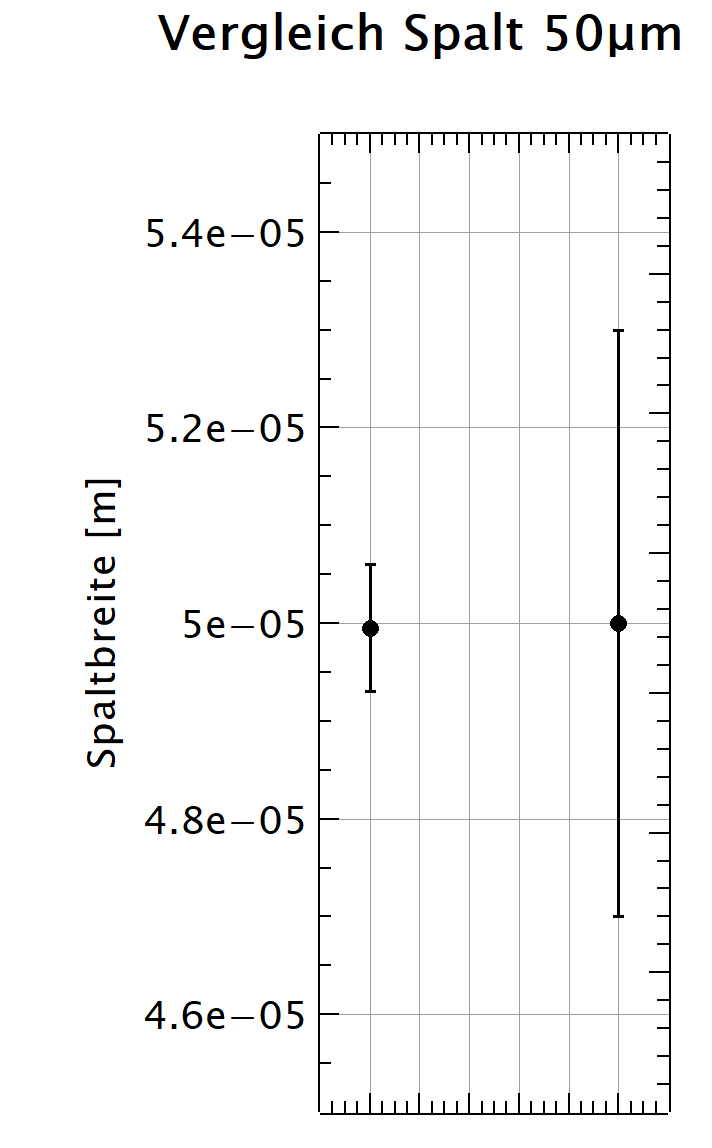
\includegraphics[width=0.4\textwidth]{data/dis_sp_50.png}
	\caption{Vergleich der gemessenen Werten mit den Theoretischen des $50\mu m$ Spalts}
	\label{fig:dis_spalt_50}
\end{figure}

\subsection*{Spalt $200\mu m$}
\begin{figure}[h!]
	\centering
	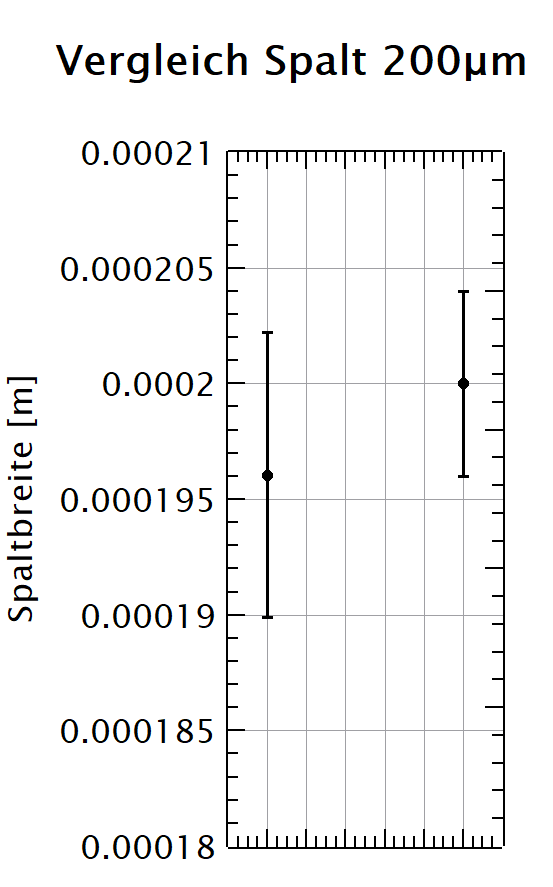
\includegraphics[width=0.4\textwidth]{data/dis_sp_200.png}
	\caption{Vergleich der gemessenen Werten mit den Theoretischen des $200\mu m$ Spalts}
	\label{fig:dis_spalt_200}
\end{figure}

\subsection*{Antispalt $0.33mm$}
\begin{figure}[h!]
	\centering
	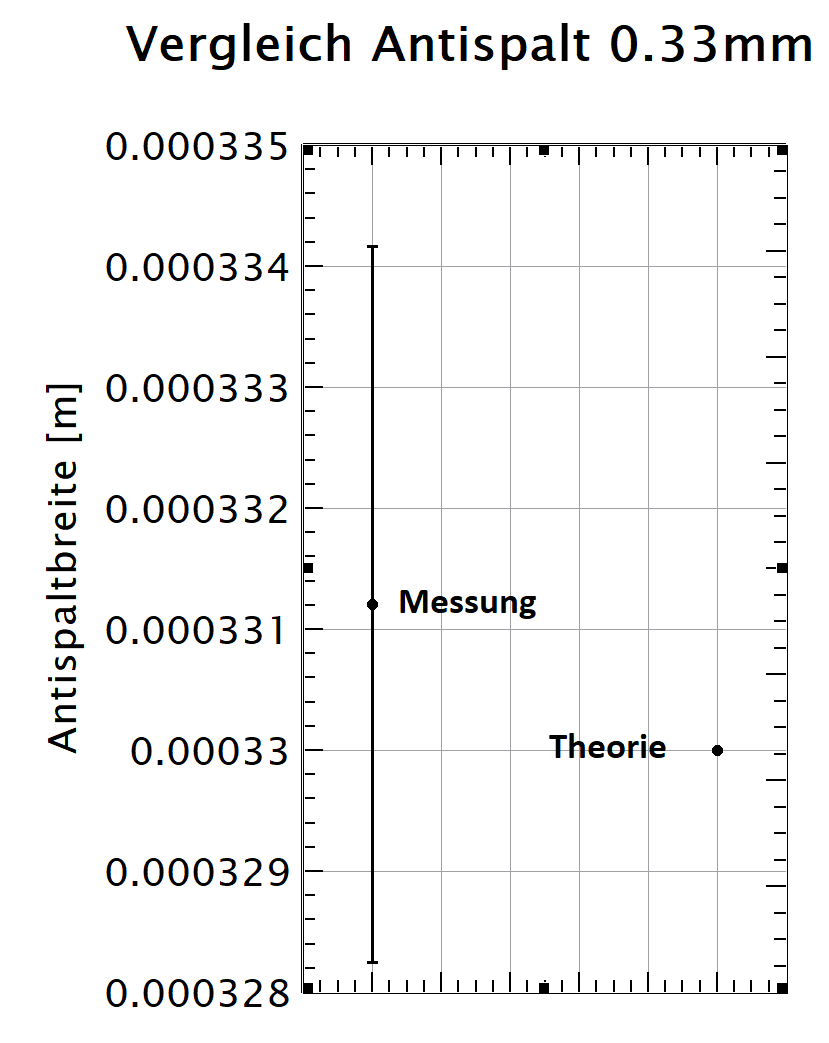
\includegraphics[width=0.4\textwidth]{data/dis_asp_33.png}
	\caption{Vergleich der gemessenen Werten mit den Theoretischen des $0.33mm$ Antispalts}
	\label{fig:dis_aspalt_33}
\end{figure}

\subsection*{Antispalt $0.124mm$}
\begin{figure}[h!]
	\centering
	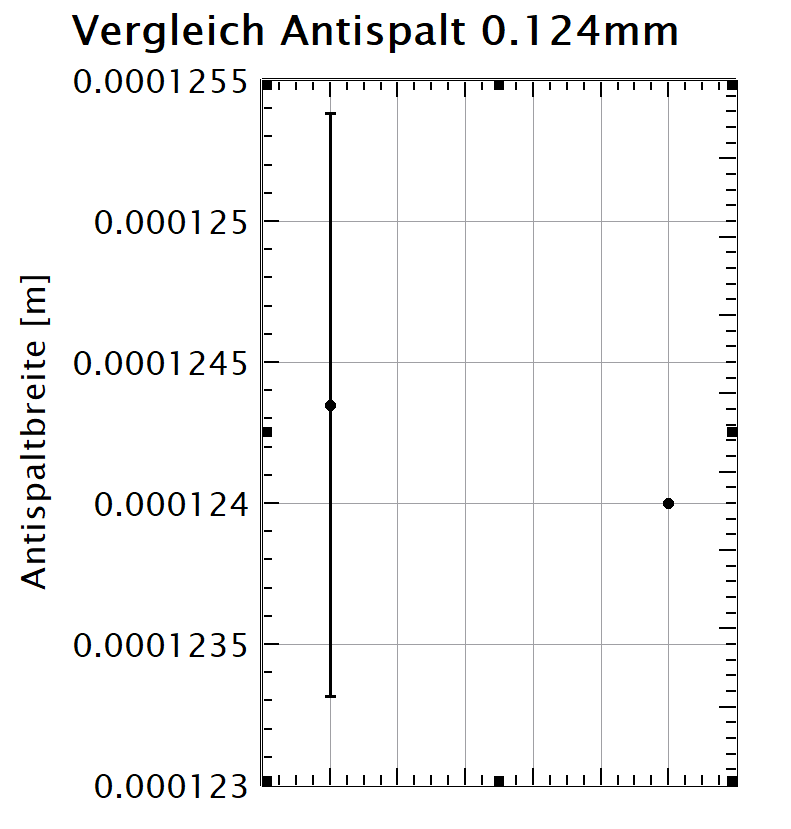
\includegraphics[width=0.4\textwidth]{data/dis_asp_12.png}
	\caption{Vergleich der gemessenen Werten mit den Theoretischen des $0.124mm$ Antispalts}
	\label{fig:dis_aspalt_12}
\end{figure}

\subsection*{Loch $150\mu m$}
\begin{figure}[h!]
	\centering
	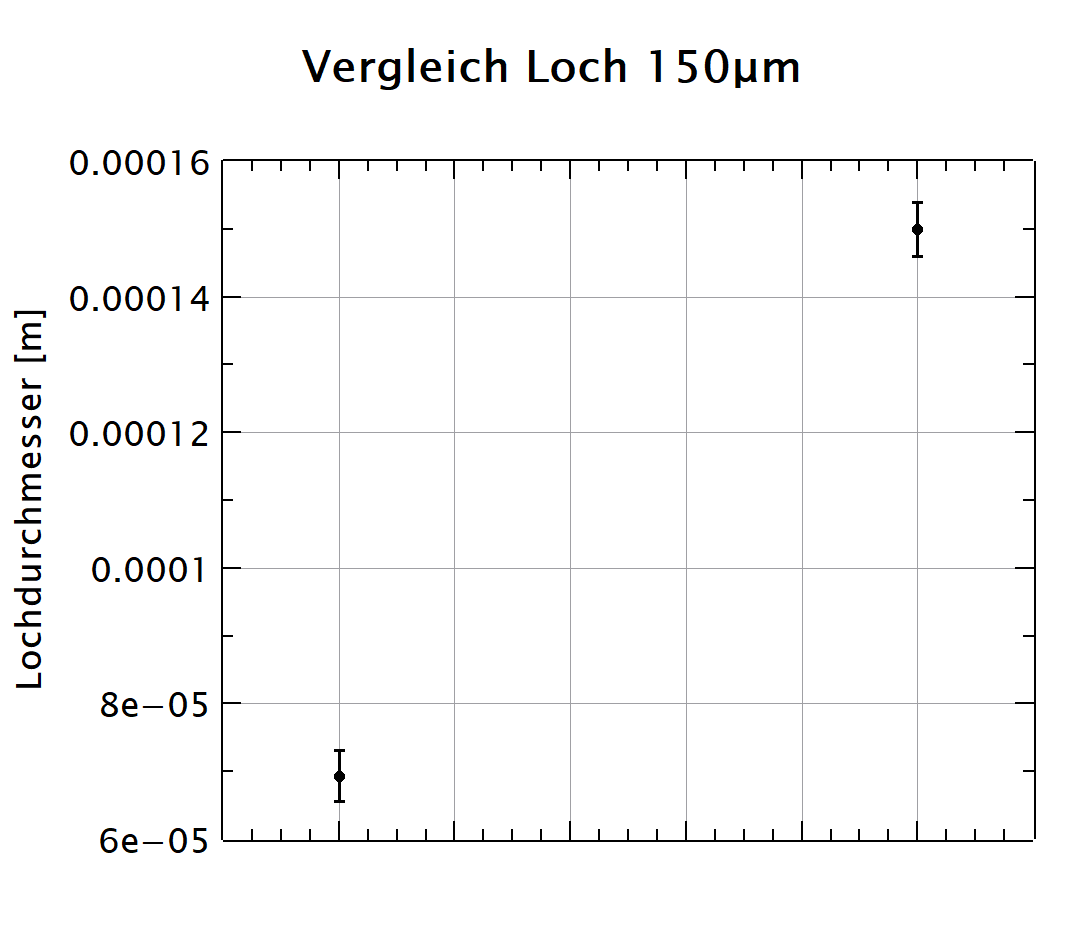
\includegraphics[width=0.4\textwidth]{data/dis_loch_150.png}
	\caption{Vergleich der gemessenen Werten mit den Theoretischen des $150\mu m$ Loch}
	\label{fig:dis_loch_150}
\end{figure}

\begin{figure}[h!]
	\centering
	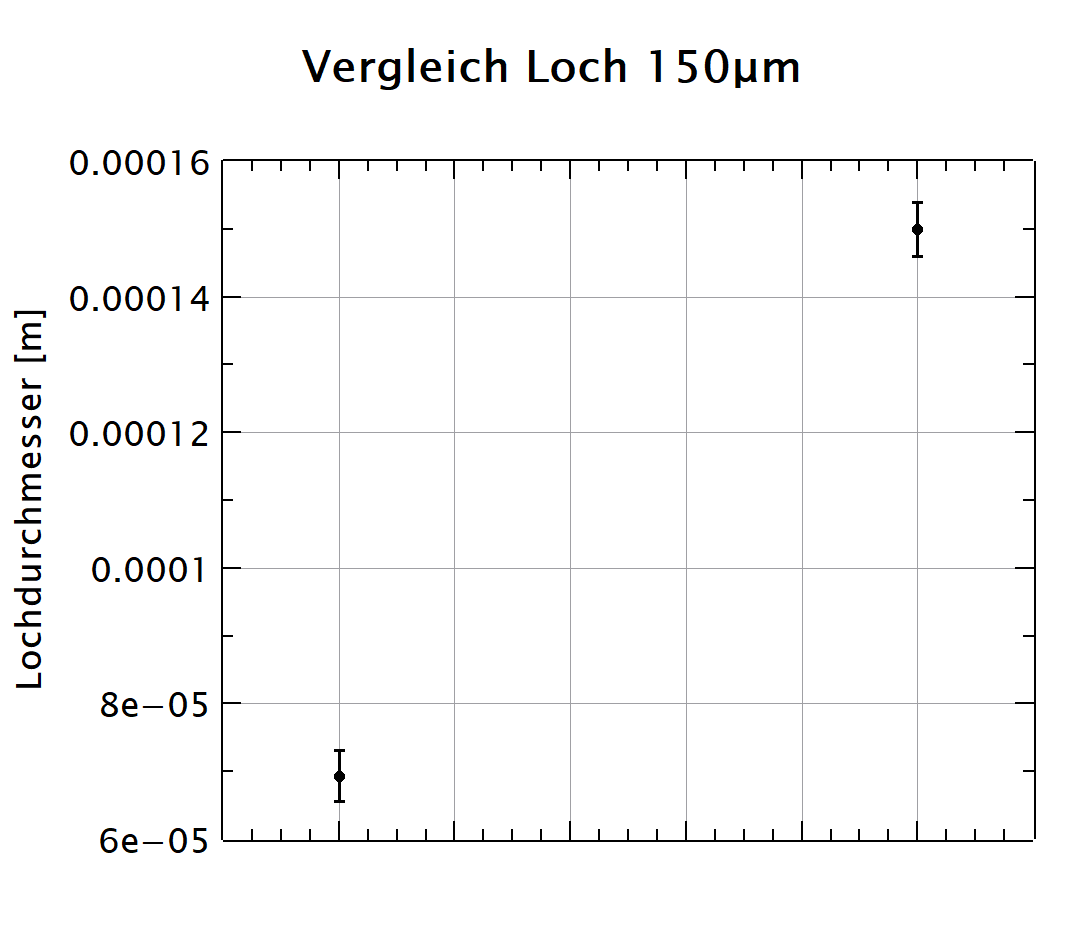
\includegraphics[width=0.4\textwidth]{data/dis_loch_150.png}
	\caption{Überprüfung des gemessenen Lochs mit Alternativer Messmethode}
	\label{fig:dis_loch_150}
\end{figure}

\subsection*{Loch $100\mu m$}
\begin{figure}[h!]
	\centering
	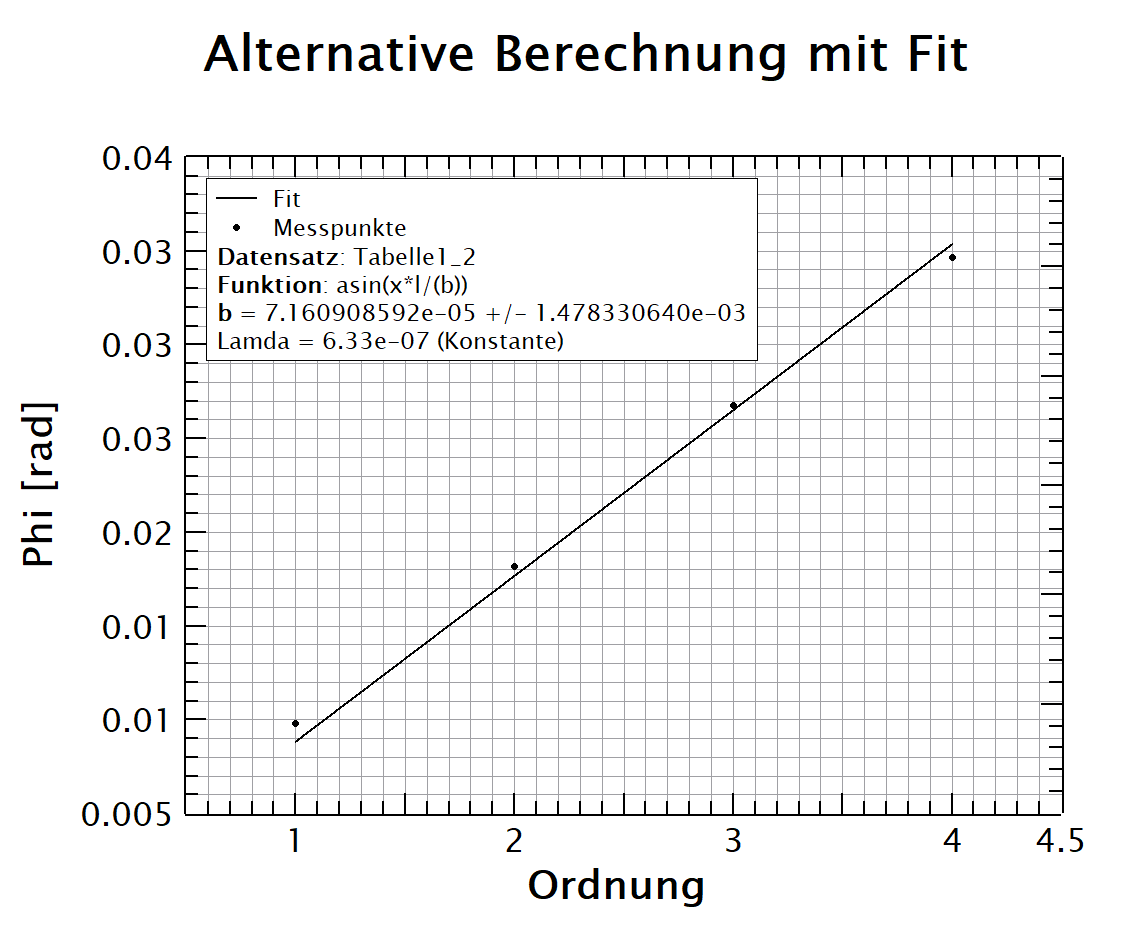
\includegraphics[width=0.4\textwidth]{data/fit_felerhaftes_loch.png}
	\caption{Vergleich der gemessenen Werten mit den Theoretischen des $100\mu m$ Loch}
	\label{fig:dis_loch_100}
\end{figure}

\subsection*{Gitter $70\mu m$}
\begin{figure}[h!]
	\centering
	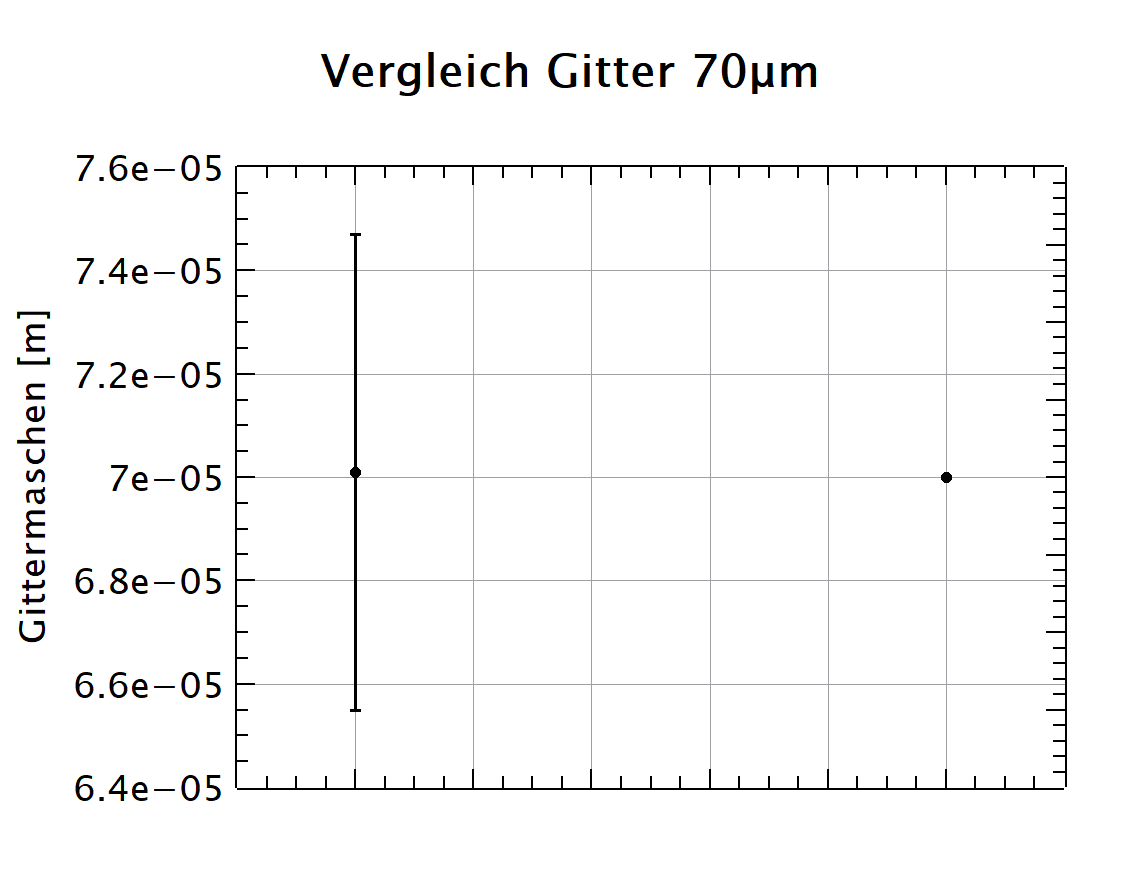
\includegraphics[width=0.4\textwidth]{data/dis_gitter.png}
	\caption{Vergleich der gemessenen Werten mit den Theoretischen des $70\mu m$ Gitter}
	\label{fig:dis_gitter}
\end{figure}

\subsection*{Doppelspalt $40\mu m$}
\begin{figure}[h!]
	\centering
	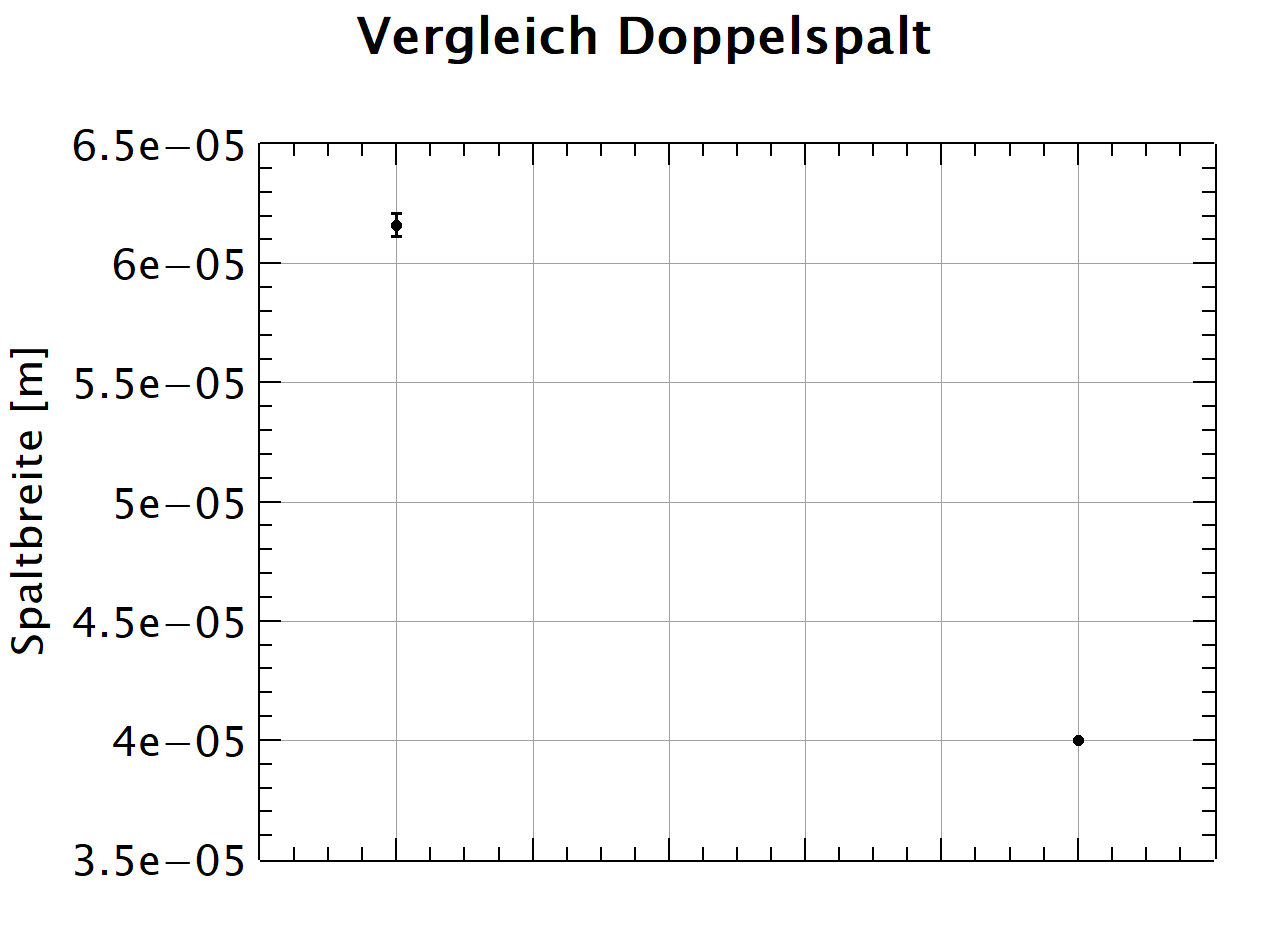
\includegraphics[width=0.4\textwidth]{data/dis_doppel.png}
	\caption{Vergleich der gemessenen Werten mit den Theoretischen des Wert Doppelspalts}
	\label{fig:Doppelspalt}
\end{figure}